\documentclass[fleqn, a4paper, 12pt]{article}
\usepackage{amsmath, amssymb, amsthm}
\usepackage{marginnote}
\usepackage{gensymb}
\usepackage{commath}
\usepackage{xcolor}
\usepackage{cancel}
\usepackage{siunitx}
\usepackage{tikz, pgfplots}
	\usetikzlibrary{calc, hobby, patterns, intersections}
\usepackage{graphicx}
\usepackage{hyperref}
\usepackage{datetime}
\usepackage{changes}
\usepackage{ulem}
\usepackage{xfrac}
\usepackage{asymptote}
\usepackage{enumerate}
\usepackage{todonotes}
\setcounter{secnumdepth}{4}
\newcommand\numberthis{\addtocounter{equation}{1}\tag{\theequation}}

\newcommand{\AxisRotator}[1][rotate=0]{%
	\tikz [x=0.25cm,y=0.60cm,line width=.2ex,-stealth,#1] \draw (0,0) arc (-150:150:1 and 1);%
}

\theoremstyle{definition}
\newtheorem{example}{Example}
\newtheorem{definition}{Definition}

\theoremstyle{theorem}
\newtheorem{theorem}{Theorem}

\newenvironment{solution}
{\begin{proof}[Solution]\let\qed\relax}
	{\end{proof}}

\newcommand{\curl}{\mathrm{curl\,}}

%\renewcommand{\int_{min}^{max}}{\int\displaylimits_{min}^{max}}

%opening
\title{Lecture 24}
\author{Aakash Jog}
\date{\formatdate{20}{1}{2015}}

\begin{document}

\maketitle
%\setlength{\mathindent}{0pt}

\tableofcontents

\newpage
\section{}

\begin{example}
	A man is pushing a box of mass $m$ on a horizontal surface, with $F = \dfrac{m g t}{\tau}$. The coefficients of friction between the box and the floor are $\mu_s$ and $\mu_k$. Find the velocity as a function of time.
\end{example}

\begin{solution}
	Case I : $t < t_0$
	\begin{align*}
		\mu_s m g &= \dfrac{m g t_0}{\tau}\\
		\therefore \mu_s &= \dfrac{t_0}{\tau}\\
		\therefore t_0 &= \mu_s \tau
	\end{align*}
	Case II : $t > t_0$
	\begin{align*}
		F_{\text{net}} &= \dfrac{m g t}{\tau} - \mu_k m g\\
		&= m g \left( \dfrac{t}{\tau} - \mu_k \right)\\
		\therefore a &= g \left( \dfrac{t}{\tau} - \mu_k \right)\\
		\therefore v &= \dfrac{g t^2}{2 \tau} - \mu_k g t + c\\
		v(\mu_s \tau) &= 0\\
		\therefore 0 &= \dfrac{g {\mu_s}^2 \tau^2}{2 \tau} - \mu_k g \mu_s \tau + c\\
		\therefore c &= \mu_s \mu_k g \tau - \dfrac{{\mu_s}^2 g \tau}{2}\\
		\therefore v &= \dfrac{g t^2}{2 \tau} - \mu_k g t + \mu_s \mu_k g \tau - \dfrac{{\mu_s}^2 g \tau}{2}
	\end{align*}
	Therefore,
	\begin{equation*}
		v = 
			\begin{cases}
				0 &;\quad t < \mu_s \tau\\
				\dfrac{g t^2}{2 \tau} - \mu_k g t + \mu_s \mu_k g \tau - \dfrac{{\mu_s}^2 g \tau}{2} &;\quad t > \mu_s \tau
			\end{cases}
	\end{equation*}
\end{solution}

\begin{example}
	A hollow sphere, a solid sphere, a hollow cylinder, and a solid cylinder of equal masses and radii are rolling without slipping down an incline of angle $\theta$. What is the minimal coefficient of static friction that will assure rolling without slipping for all bodies?
\end{example}

\begin{solution}
	About the centre of mass,
	\begin{align*}
		m g \sin \theta - f &= m a\\
		k m R^2 \alpha &= f R\\
		\therefore m g \sin \theta - k m a &= m a\\
		\therefore a &= \dfrac{g \sin \theta}{k + 1}\\
		\therefore f &= k m a\\
		&= \dfrac{k}{k + 1} m g \sin \theta
	\end{align*}
	Therefore, 
	\begin{align*}
		f_s &\leq \mu m g \cos \theta\\
		\therefore \mu_{\text{min}} &= \dfrac{1}{2} \tan \theta
	\end{align*}
\end{solution}

\begin{example}
	A system of a mass $m$ and two springs of spring constant $k$ is arranged as shown. It is submerged in a fluid such that $\overrightarrow{f} = - \gamma \overrightarrow{v}$. Assuming there is no under-damping, what should be $k$ for the mass to return to a point near the origin in minimal time?\\
	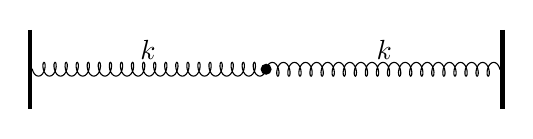
\begin{tikzpicture}
		\def\l{3};
		\def\x{0};
		\def\h{1};
		\def\segmentlength{4};
		
		\begin{scope}
		\fill (0,0) circle [radius = 2pt];
		\end{scope}
		
		\begin{scope}
		\draw [decorate, decoration = {coil, segment length = {(\l + \x)/(\l)*\segmentlength}}] (0,0) -- (\l,0) node [midway, above] {$k$};
		\draw [decorate, decoration = {coil, segment length = {(\l + \x)/(\l)*\segmentlength}}] (0,0) -- (-\l,0) node [midway, above] {$k$};
		\end{scope}
		
		\begin{scope}[ultra thick]
		\draw (-\l,{\h/2}) -- (-\l,{-\h/2});
		\draw (\l,{\h/2}) -- (\l,{-\h/2});
		\end{scope}
	\end{tikzpicture}
\end{example}

\begin{solution}
	\begin{align*}
		F &= - 2 k x - \gamma \dot{x}\\
		\therefore m \ddot{x} &= -\gamma \dot{x} - 2 k x\\
		\therefore \ddot{x} + \dfrac{\gamma}{m} \dot{x} + \dfrac{2 k}{m} x &= 0
	\end{align*}
	Therefore, for minimal $k$, there must be critical damping
	\begin{align*}
		\left( \dfrac{\gamma}{m} \right)^2 - 4 \left( \dfrac{2k}{m} \right) = 0\\
		\therefore k &= \dfrac{\gamma^2}{8m}
	\end{align*}
\end{solution}

\begin{example}
	Two rockets start from the same point in space with zero velocity.\\
	The first rocket moves in the $x$ direction, with initial mass $m_0$. It releases gas with rate $\lambda$, with velocity $v_0$ with respect to it.\\
	The second rocket moves at $30 \degree$ with respect to the $y$ direction. It releases gas with velocity $v_0$ with respect to it. Its mass changes as
	\begin{equation*}
		m(t) = m_0 e^{- \alpha t}
	\end{equation*}\\
	What is the magnitude of acceleration of rocket 2 with respect to rocket 1, at $t = \dfrac{1}{\alpha}$?
\end{example}

\begin{solution}
	For rocket 1,
	\begin{align*}
		\dod{p}{t} &= m \dod{v}{t} + v_0 \dod{m}{t}\\
		\therefore 0 &= (m_0 - \lambda t) a_1 - v_0 \lambda\\
		\therefore a_1 &= \dfrac{v_0 \lambda}{m_0 - \lambda t}
	\end{align*}
	For rocket 2,
	\begin{align*}
		\dod{p}{t} &= m \dod{v}{t} + v_0 \dod{m}{t}\\
		\therefore - &= m_0 e^{-\alpha t} a_2 - v_0 \left( \alpha m_0 e^{-\alpha t} \right)\\
		\therefore a_2 &= \alpha v_0
	\end{align*}\\
	Therefore,
	\begin{align*}
		\overrightarrow{a_1} &= \left( \dfrac{v_0 \lambda}{m_0 - \lambda t} , 0 \right)\\
		\overrightarrow{a_2} &= \left( \dfrac{1}{2} \alpha v_0 , \dfrac{\sqrt{3}}{2} \alpha v_0 \right)
	\end{align*}
	Therefore,
	\begin{align*}
		a_{2,1} &= \sqrt{\left( \dfrac{1}{2} \alpha v_0 - \dfrac{v_0 \alpha}{m_0 - \sfrac{\lambda}{\alpha}} \right)^2 + \left( \dfrac{\sqrt{3}}{2} \alpha v_0 \right)^2}
	\end{align*}
\end{solution}

\begin{example}
	A thin cylinder of radius $R$ is filled with a gas and is fixed at its centre. Its initial mass is $m_0$. Gas is emitted with velocity $u$ with respect to the cylinder, with mass rate of emission $c$. Find the angular velocity of the cylinder.
	\begin{tikzpicture}
		\def\R{3};
		\def\angle{30};
		
		\draw (0,0) circle [radius = \R];
		\draw [-stealth] (\angle:\R) -- ++({-(90 - \angle)} : 2) node [below right] {gas emission};
	\end{tikzpicture}
\end{example}

\begin{solution}
	About the centre,
	\begin{align*}
		L(t) &= \dfrac{1}{2} (m + \dif m) R^2 \omega + R (\dif m) \omega\\
		L(t + \dif t) &= \dfrac{1}{2} (m + \dif m) R^2 (\omega + \dif \omega) R^2 + (-\dif m) (\omega R - u) R\\
		\therefore \dod{L}{t} &= \dfrac{\dfrac{1}{2} (m + \dif m) R^2 \dif \omega + \dif m R u}{\dif t}\\
		\therefore 0 &= \dfrac{1}{2} m R^2 \dod{\omega}{t} + \dod{m}{t} R u\\
		&= \dfrac{1}{2} (m_0 - c t) R^2 \dod{\omega}{t} - c R u\\
		\therefore (m_0 - c t) R^2 \dod{\omega}{t} &= 2 c R u\\
		\therefore \dif \omega &= \dfrac{2 c u \dif t}{R (m_0 - c t)}\\
		\therefore \omega &= \dfrac{2 u}{R} \ln \dfrac{m_0}{m_0 - c t}
	\end{align*}
\end{solution}

\begin{example}
	Two birds are sitting on a square body with sides of length $2a$ and mass density $\sigma$. Bird A flies away in the negative $x$ direction and Bird B files away at $30\degree$, towards the positive $x$ direction, with respect to the $y$ direction. Find the velocity of the centre of the square and the angular velocity of the square.\\
	\begin{tikzpicture}
		\def\a{2};
		\def\angle{30};
		\def\F{1};
		
		\coordinate (mass A) at (-\a,0);
		\coordinate (mass B) at (\a,0);
		
		\begin{scope}[stealth-stealth, lightgray]
			\draw ({-(\a + 1)},0) -- ({(\a + 1)},0) node [right] {$x$};
			\draw (0,{-(\a + 1)}) -- (0,{(\a + 1)}) node [above] {$y$};
		\end{scope}
		
		\fill (0,0) circle [radius = 1pt] node [above right] {D};
		
		\draw (-\a,-\a) rectangle (\a,\a);
		\fill (mass A) circle [radius = 2pt] node [above right] {A};
		\fill (mass B) circle [radius = 2pt] node [above left] {B};
		
		\begin{scope}[-stealth]
			\draw (mass A) -- ++(-90:\F) node [left] {$v_0$};
			\draw (mass B) -- ++({90 - \angle}:\F) node [right] {$v_0$};
		\end{scope}
	\end{tikzpicture}
\end{example}

\begin{solution}
	By COLM in the $y$ direction,
	\begin{align*}
		0 &= -m v_0 + m v_0 \cos \alpha + 4 a^2 \sigma {v_D}_y\\
		\therefore 4 a^2 \sigma {v_D}_y &= m v_0 (1 - \cos \alpha)\\
		\therefore {v_D}_y &= \dfrac{m v_0 (1 - \cos \alpha)}{4 a^2 \sigma}
	\end{align*}
	By COLM in the $x$ direction,
	\begin{align*}
		-4 a^2 \sigma {v_D}_x &= m v_0 \sin \alpha\\
		\therefore {v_D}_x &= -\dfrac{m v_0 \sin \alpha}{4 a^2 \sigma}
	\end{align*}
	Therefore,
	\begin{align*}
		v_D &= - \dfrac{m v_0 \sin \alpha}{4 a^2 \sigma} \hat{i} + \dfrac{m v_0 (1 - \cos \alpha)}{4 a^2 \sigma} \hat{j}
	\end{align*}
	By COAM,
	\begin{align*}
		m v_0 a + m v_0 \cos \alpha a &= I \omega\\
		\therefore \omega &= \dfrac{m v_0}{I} (1 + \cos \alpha)\\
		&= \dfrac{m v_0}{\dfrac{8}{3} \sigma a^4} (1 + \cos \alpha)\\
		&= \dfrac{3 m v_0}{8 \sigma a^4} (1 + \cos \alpha)
	\end{align*}
	$\omega$ is clockwise.
\end{solution}

\begin{example}
	A thin box with walls of length $a$ and mass $m$, each, is placed on a surface. A point cat is at the bottom right corner of the box. The cat jumps up towards the left at an angle $\alpha$ with the horizontal, with velocity $v$. Assuming there is no friction, find the velocity of the box while the cat is in the air. On reaching the other side, the cat clings to the wall. Assuming no friction, find the height the cat reaches. If friction is infinite, find the height. Consider $v_0$ and $\alpha$ to be such that the cat reaches the wall at height $\dfrac{a}{2}$. Assuming the friction to be inifinite, find $v_0$ such that the box does not topple.
\end{example}

\begin{solution}
	By COLM in the horizontal direction,
	\begin{align*}
		0 &= - m v_0 \cos \alpha + 4m v\\
		\therefore v &= \dfrac{v_0 \cos \alpha}{4}
	\end{align*}
	\begin{align*}
		(v_{\text{cat, box}})_x &= \dfrac{5}{4} v_0 \cos \alpha\\
		\therefore a &= \dfrac{5}{4} v_0 \cos \alpha t\\
		\therefore t &= \dfrac{4 a}{5 v_0 \cos \alpha}
	\end{align*}
	Therefore,
	\begin{align*}
		y &= v_0 \sin \alpha t - \dfrac{1}{2} g t^2\\
		&= v_0 \sin \alpha \cdot \dfrac{4 a}{5 v_0 \cos \alpha} - \dfrac{1}{2} g \dfrac{16 a^2}{9 {v_0}^2 \cos^2 \alpha}\\
		&= \dfrac{4 a \tan \alpha}{5} - \dfrac{8 a^2 g}{25 {v_0}^2 \sec^2 \alpha}
	\end{align*}
	If the friction is infinite,
	\begin{align*}
		a &= v_0 \cos \alpha t\\
		\therefore t &= \dfrac{a}{\cos \alpha}\\
		\therefore y &= v_0 \sin \alpha t - \dfrac{1}{2} g t^2\\
		&= v_0 \sin \alpha \dfrac{a}{\cos \alpha} - \dfrac{1}{2} g \dfrac{a^2}{\cos^2 \alpha}\\
		&= v_0 a \tan \alpha - \dfrac{a^2 g \sec^2 \alpha}{2}
	\end{align*}
	After the collision, the box rotates about point A, i.e. the lower left corner.\\
	\begin{tikzpicture}
		\def\a{6};
		
		\begin{scope}[dashed]
			\draw ({-\a/2 },0) -- ({\a/2},0);
			\draw (0,{-\a/2}) -- (0,{\a/2});
		\end{scope}
		
		\coordinate (COM) at ({-\a/10},0);
		\coordinate (cat) at (-\a/2,0);
		
		\fill (COM) circle [radius = 2 pt] node [above] {COM};
		\fill (cat) circle [radius = 2 pt] node [above right] {cat};
		
		\draw (-\a/2,-\a/2) rectangle (\a/2,\a/2);
	\end{tikzpicture}\\
	\begin{tikzpicture}[rotate = 40]
		\def\a{6};
		
		\begin{scope}[dashed]
			\draw ({-\a/2 },0) -- ({\a/2},0);
			\draw (0,{-\a/2}) -- (0,{\a/2});
		\end{scope}
		
		\coordinate (COM) at ({-\a/10},0);
		\coordinate (cat) at (-\a/2,0);
		
		\fill (COM) circle [radius = 2 pt] node [above] {COM};
		\fill (cat) circle [radius = 2 pt] node [above right] {cat};
	
		\draw (-\a/2,-\a/2) rectangle (\a/2,\a/2);
	\end{tikzpicture}\\
	At the instant of collision, angular momentum is conserved. After that, linear and angular momenta are not conserved, but mechanical energy is conserved.\\
	By COAM at the time of collision, about the lower left corner,
	\begin{align*}
		\dfrac{a}{2} m v_0 \cos \alpha &= I_A \omega\\
		\therefore \dfrac{a}{2} m v_0 \cos \alpha &= \left( 2 \cdot \dfrac{1}{2} m a^2 + 2 \left( \dfrac{1}{12} m a^2 + m \left( a^2 + \dfrac{a^2}{4} \right) \right) + m \left( \dfrac{a}{2} \right)^2 \right) \omega
	\end{align*}
\end{solution}

\begin{example}
	A body with moment of inertia $I_0$, radius $R$ and mass $m$ is rolling on a surface with $v_0 = \omega_0 R$. The air friction is given by $\overrightarrow{f_a} = - \gamma \overrightarrow{v}$. Assume $\mu m g > \gamma v_0$ Find all forces acting on the body. Find the friction due to the ground, as a function of $v$. Find the velocity of the centre of mass as a function of time.\\
	\begin{tikzpicture}
		\def\R{4};
		\def\F{1};
		
		\draw (0,0) circle [radius = \R];
		
		\draw (-\R,-\R) -- (\R,-\R);
		
		\begin{scope}[-stealth]
			\draw (0,{\F/2}) arc (90:-180:{\F/2}) node [left] {$\omega$};
			\draw (0,0) -- (0:\F) node [right] {$v$};
		\end{scope}
	\end{tikzpicture}
\end{example}

\begin{solution}
	~\\
	\begin{tikzpicture}
		\def\R{4};
		\def\F{1};
		
		\draw (0,0) circle [radius = \R];
		
		\draw (-\R,-\R) -- (\R,-\R);
		
		\begin{scope}[-stealth]
			\draw (0,{\F/2}) arc (90:-200:{\F/2}) node [right] {$\omega$};
			\draw (0,0) -- (0:\F) node [right] {$v$};
		\end{scope}
		
		\begin{scope}[-stealth, red]
			\draw (0,0) -- ++(-90:\F) node [below] {$mg$};
			\draw (0,-\R) -- ++(90:\F) node [above] {$N$};
			\draw (0,0) -- ++(180:\F) node [above] {$f_a$};
			\draw (0,-\R) -- ++(0:\F) node [below] {$f_s$};
		\end{scope}
	\end{tikzpicture}\\
	\begin{align*}
		m a &= f_a - f_s\\
		\therefore m a &= \gamma v - f_s
	\end{align*}
	\begin{align*}
		I_0 \alpha &= f_s R
	\end{align*}
	As the body is purely rolling,
	\begin{align*}
		a &= \alpha R
	\end{align*}
\end{solution}

\end{document}
